\documentclass[handout]{beamer}

\usepackage{Haust2016glærur}

\title{Stærðfræðimynstur í tölvunarfræði}
\subtitle{Vika 6, seinni fyrirlestur}

\begin{document}

\begin{frame}
\titlepage
\end{frame}


\section{Inngangur}

\begin{frame}{Í síðasta tíma}
    \begin{itemize}
        \item Leifajöfnur
        \item Dulkóðun
    \end{itemize}
\end{frame}

\section{Þrepasannanir (5.1)}

\begin{frame}{Hugmyndin}
    \begin{columns}
        \column{0.5\textwidth}
        \begin{itemize}
            \item Getum við klifrað upp óendanlegan stiga?
            \item Getum sannfært okkur um að við komumst í hvaða þrep sem er ef
            \begin{enumerate}
                \item Við komumst í fyrsta þrep stigans
                \item Ef við komumst í tiltekið þrep stigans komumst við í næsta þrep
            \end{enumerate}
        \end{itemize}
        \column{0.5\textwidth}
        \begin{center}
            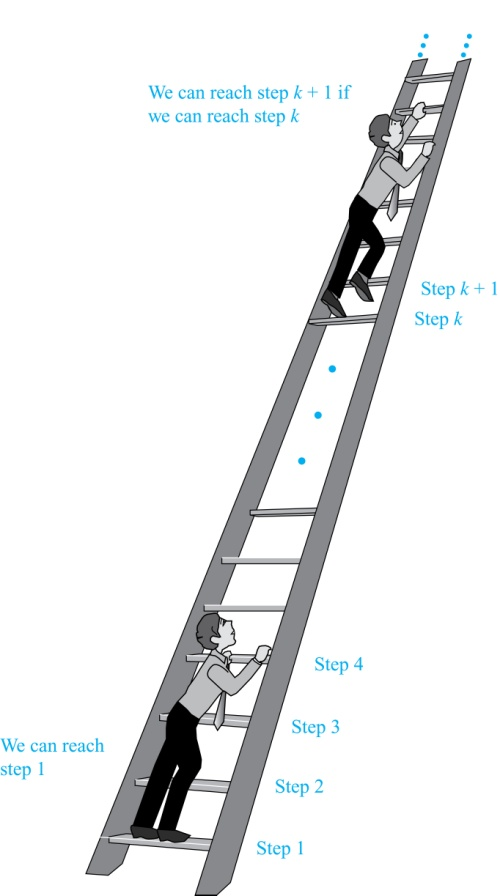
\includegraphics[width=0.8\linewidth]{induction-stairs}
        \end{center}
    \end{columns}
\end{frame}

\begin{frame}{Skilgreiningar}
    \begin{tcolorbox}[title=Sönnun með þrepun]
        Til að sanna að fyrir umsögn $P$ að $P(n)$ gildi fyrir allar jákvæðar heiltölur $n$ er nægjanlegt að framkvæma tvö skref:
        \begin{itemize}
            \item Grunnskref (e. \emph{basis step}): Sannreynum að $P(1)$ sé satt
            \item Þrepunarskref (e. \emph{inductive step}): Sýnum að afleiðingin $P(k) \to P(k+1)$ sé sönn fyrir allar jákvæðar heiltölur $k$
        \end{itemize}
    \end{tcolorbox}
    Í þrepuninni gerum við ráð fyrir að $P(k)$ sé satt fyrir ótiltekna heiltölu $k$ og sönnum að $P(k+1)$ sé satt. Þá er $P(k)$ þrepunarforsendan (e. \emph{inductive hypothesis}).
\end{frame}

\begin{frame}{Sönnun summuformúlu með þrepun}
    Notum þrepun til að sýna að sé $n$ jákvæð heiltala, þá sé
    \[
        1 + 2 + \ldots + n = \frac{n(n+1)}{2}
    \]
    \pause
    (Example 1 í kafla 5.1 í bók)
\end{frame}

\begin{frame}{Nokkur mikilvæg atriði}
    \begin{itemize}
        \item Við getum sett grunnregluna um þrepun fram sem röksemdareglu sem gildir fyrir allar umsagnir $P$ sem hafa mengi jákvæðra heiltalna sem óðal
        \[
            \left(P(1) \land \forall k: (P(k) \to P(k+1))\right) \to \forall n: P(n)
        \] \pause
        \item Í þrepuninni er þrepunarforsendan ekki að staðhæfingin gildi fyrir allar jákvæðar heiltölur, heldur að hún gildi fyrir einhverja tölu $k$ og að hún gildi þá líka fyrir næstu tölu, $k+1$ \pause
        \item Þrepunarsannanir þurfa ekki að byrja í heiltölunni 1, getum byrjað í heiltölu $b$ og sýnt fram á að eitthvað gildi fyrir heiltölur $\geq b$
    \end{itemize}
\end{frame}

\begin{frame}{Af hverju virkar þrepun?}
    \begin{itemize}
        \item Þrepun virkar vegna frumsendu um velröðun (e. \emph{well-ordering}) jákvæðu heiltalnanna
        \begin{itemize}
            \item Sérhvert hlutmengi í jákvæðu heiltölunum sem ekki er tómt hefur minnsta stak
            \item Fjallað um í viðauka 1
        \end{itemize}
        \item Getum þá sannað með mótsögn
    \end{itemize}
\end{frame}

\begin{frame}{Af hverju virkar þrepun?}
    \begin{itemize}
        \item Látum $P(1)$ vera satt og $P(k) \to P(k+1)$ vera satt fyrir allar jákvæðar heiltölur $k$ en að til sé jákvæð heiltala $n$ svo að $P(n)$ sé ósatt
        \item Þá er mengi þeirra heiltalna sem gerir $P(n)$ ósatt ekki tómt og hefur þar með minnsta stak, sem við köllum $m$ \pause
        \begin{itemize}
            \item $m$ getur ekki verið 1, því $P(1)$ er satt \pause
            \item $m$ er jákvætt og hærra en 1, so $m-1$ er jákvæð heiltala \pause
        \end{itemize}
        \item $m-1$ er minna en $m$, svo $P(m-1)$ er satt \pause
        \item Þar sem $P(m-1) \to P(m)$ er satt hlýtur $P(m)$ þá að vera satt \pause
        \item Mótsögn í vali á $m$, $P(n)$ er satt fyrir allar jákvæðar heiltölur $n$ 
    \end{itemize}
\end{frame}

\begin{frame}{Takmarkanir þrepunar}
    \begin{itemize}
        \item Kostur við þrepun er að hún býður upp á kerfisbundna leið til að sannreyna tilgátur
        \item Galli við þrepun er að við þurfum að vera með hugmynd að tilgátu til að staðfesta áður en hafist er handa
        \item Takmörkuð innsýn fæst í vandamálið
    \end{itemize}
\end{frame}

\section{Þrepunardæmi}

\begin{frame}{Summa fyrstu n jákvæðu oddatalnanna}
    \begin{itemize}
        \item Getum við giskað á formúlu fyrir $1+3+5+\ldots +(2n-1)$?
        \begin{itemize}
            \item $1=1$, $1+3=4$, $1+3+5=9$, $1+3+5+7=16$, $\ldots$\pause
        \end{itemize}
        \item Giskum á að $\sum_{i=1}^n(2i-1)=n^2$, látum $P(n)$ vera þá staðhæfingu að formúlan haldi fyrir allar jákvæðar heiltölur $n$
        \item Sönnum með þrepun
        \begin{itemize}
            \item Example 2 í kafla 5.1
        \end{itemize}
    \end{itemize}
\end{frame}

\begin{frame}{Sönnun á ójöfnu}
    \begin{itemize}
        \item Notum þrepun til að sanna að $n < 2^n$ fyrir allar jákvæðar heiltölur $n$
        \item Example 5 í kafla 5.1 í bók
    \end{itemize}
\end{frame}

\begin{frame}{Sönnun á deilanleika}
    \begin{itemize}
        \item Notum þrepun til að sanna að $n^3-n$ er deilanlegt með 3 fyrir allar jákvæðar heiltölur $n$
        \item Example 8 í kafla 5.1 í bók
    \end{itemize}
\end{frame}

\begin{frame}{Sönnun á fjölda hlutmengja}
    \begin{itemize}
        \item Notum þrepun til að sanna setningu um fjölda hlutmengja endanlegs mengis
        \item Látum $P(n)$ tákna fullyrðinguna ``mengi með $n$ stök hefur $2^n$ hlutmengi''
        \item Example 10 í kafla 5.1 í bók
    \end{itemize}
\end{frame}

\begin{frame}{Sönnun á fjölda hlutmengja}
    \begin{itemize}
        \item Grunnur: Mengi með 0 stök er tóma mengið sem hefur einungis eitt ($=2^0$) hlutmengi, tóma mengið sjálft.
        \item Þrepun:
        \begin{itemize}
            \item Þrepunarforsenda: G.r.f.a. mengi $S$ með $n$ stök hafi $2^n$ hlutmengi
            \begin{itemize}
                \item Viljum sanna að mengi með $n+1$ stak hafi $2^{n+1}$ hlutmengi
            \end{itemize}
            \item Þrepunarskref: Látum $T$ vera mengi með $n+1$ stak og $S$ mengi með $n$ stök. Getum skrifað $T = S \cup \{a\}$ fyrir sérhvert $a \in T$. Þá inniheldur hvert hlutmengi $T$ stakið $a$ eða ekki. Fyrir hvert hlutmengi $X$ í $T$ sem inniheldur $a$ er til eitt hlutmengi $X - \{a\}$ sem inniheldur ekki $a$. En öll hlutmengi í $T$ sem ekki innihalda $a$ eru líka hlutmengi $S$. Fjöldi hlutmengja $T$ er þá tvöfaldur fjöldi hlutmengja $S$, sem skv. þrepunarforsendu er $2 \cdot 2^n = 2^{n+1}$, sem sanna átti 
        \end{itemize}
    \end{itemize}
\end{frame}

\begin{frame}{Ráðlögð uppbygging}
Auðvelt er að gera mistök þegar þrepasönnun er skrifuð. Ráðlögð uppbygging er:

\vspace{0.5cm}

\textbf{Setning:} Fyrir öll $n \geq b$ gildir $P(n)$

\textbf{Sönnun með þrepun:}
\begin{itemize}
    \item Grunnur: Sýnum að $P(b)$ gildir
    \item Þrepun: 
    \begin{itemize}
        \item Þrepunarforsenda: Gerum ráð fyrir að $P(n)$ gildi fyrir eitthvert $n \geq b$, viljum sanna $P(n+1)$
        \item Þrepunarskref: Notum $P(n)$ til að sanna að $P(n+1)$ gildir
    \end{itemize}
\end{itemize}
\end{frame}

\section{Sterk þrepun (5.2)}

\begin{frame}{Sterk þrepun}
\begin{itemize}
    \item Sterk þrepun er sönnunaraðferð sem er jafngild ``venjulegri'' þrepun
    \begin{itemize}
        \item Þ.e.a.s. ef hægt er að nota aðra sönnunaraðferðina má nota hina líka
    \end{itemize}
    \item Þá er ekki sýnt fram á að $P(k) \to P(k+1)$, heldur að \[[P(1) \land P(2) \land \ldots \land P(k)] \to P(k+1)\]
    \item Sterka þrepun er betra að nota þegar ljósara er að $[P(1) \land \ldots \land P(k)] \to P(k+1)$ heldur en að einungis $P(k) \to P(k+1)$
\end{itemize}
\end{frame}

\begin{frame}{Þáttun prímtalna}
    Höfum séð staðreynd um þáttun prímtalna, hluti af ``the fundamental theorem of arithmetic'':

    \begin{tcolorbox}
        Hver heiltala stærri en 1 er prímtala eða margfeldi tveggja eða fleiri prímtalna
    \end{tcolorbox}

    Getum sannað hana með sterkri þrepun.
\end{frame}

\begin{frame}{Þáttun prímtalna}
    \begin{itemize}
        \item Grunnur: Fyrir $n=2$ gildir setningin því 2 er prímtala
        \item Þrepun:
        \begin{itemize}
            \item Þrepunarforsenda: G.r.f.a. fyrir sérhvert $n \geq 2$ sé hægt að rita sérhverja heiltölu $k$ þannig að $1 < k \leq n$ sem margfeldi primtalna. \pause
            \item Þrepunarskref: Skoðum $n+1$. Ef $n+1$ er prímtala þarf ekkert að sanna. Ef $n+1$ er ekki prímtala er skv. skilgreiningu hægt að rita $n +1 = x\cdot y$, þar sem $x$ og $y$ eru jákvæðar heiltölur. Bæði $x$ og $y$ eru þá minni en $n+1$. Skv. þrepunarforsendu er þá hægt að rita bæði $x$ og $y$ sem margfeldi prímtalna og þá má rita $n+1$ sem margfeldi sömu prímtalna.
        \end{itemize}
    \end{itemize}
\end{frame}


\begin{frame}{Næst}
Talning (6.1) og skúffureglan (6.2)
\end{frame}


\end{document}
